\documentclass[12pt, letterpaper]{article}
\usepackage[utf8]{inputenc}
\usepackage[backend=biber]{biblatex}
\usepackage{float}
\usepackage{tikz}
\usepackage{hyperref}
\usepackage[newfloat]{minted}
\usepackage{caption}
\usepackage{dirtree}
\tolerance=1
\emergencystretch=\maxdimen
\hyphenpenalty=10000
\hbadness=10000
\addbibresource{references.bib}

\newenvironment{code}{\captionsetup{type=listing}}{}
\SetupFloatingEnvironment{listing}{name=Source Code}

\graphicspath{{img/}}

\title{MapReduce‐System (37)}
\author{Fabian Kleinrad (07), 5BHIF}
\date{March 2022}

\begin{document}

\begin{titlepage}
\maketitle
\end{titlepage}

\tableofcontents
\newpage

\section{Introduction}

In this project, the technology MapReduce is being simulated. Thereby a simple system has been developed to imitate the functionality of a MapReduce application. All of the functionality in this project is written with C++17 and compiled with the help of the meson build system\footfullcite{meson}. The communication is based on the TCP protocol and realized using the C++ library asio\footfullcite{asio}.\newline
Furthermore, to increase performance and usability, protocol buffers\footfullcite{protobuf} are utilized. Protocol Buffers enable the serialization of data structures in an efficient manner, which simplifies working with messages sent between parties in the MapReduce system.\newline
To make use of the advantages of a MapReduce architecture, a simple use-case consisting of counting the number of character occurrences in a plain text document has been implemented. This kind of application was chosen due to its simplicity, which enables the focus of this project to stay on MapReduce rather than a test application. 

\section{MapReduce}

MapReduce is a programming model developed to decrease the computational time of large data sets. It was invented by Google, the reason being the need to compute various kinds of derived data. Examples would be inverted indices or representations of the graph structure of web documents. These applications all have simplicity in common. There are no complex operations needed to accomplish said tasks. Furthermore, these kinds of processes are characterized by accepting large amounts of input data and reducing it to a fraction of itself. MapReduce presents a solution to parallelization, fault-tolerance, data distribution, and load balancing. It is based on the principle of map and reduce, which is eponymous for the technology.\footfullcite{mapreducePaper}

\subsection{Input Data}

MapReduce processes unstructured or semi-structured data. The system is designed to accept large amounts of data in bulk. In the first step of the MapReduce process, this data is split into subsets to allow for data distribution. The way this data is divided depends on the implementation and the type of input data present. The result of splitting the raw data is a set of key/value pairs.\footfullcite{uniLeibzigMapReduce}

\subsection{Map}

The map function accepts a set of key/value pairs, with the implementation being provided by the user. The result of this phase is once more a set of key/value pairs. These result pairs represent the significant information contained in the input data. These significant data pairs directly influence the result, and all unneeded information is discarded. The name map stems from assigning a quantity attribute representing the value of the resulting pairs to a quality attribute.\footcite{uniLeibzigMapReduce}\footcite{mapreducePaper}

\subsection{Reduce}

Sorted key/value pairs get passed to the reduce function, which groups and reduces the set of data points. The logic of this grouping functionality depends on the application of MapReduce. For that reason, the reduce function is also implemented by the user.\footcite{uniLeibzigMapReduce}

\pagebreak

\subsection{Additional Phases}

\subsubsection{Shuffle}
In most implementations of a MapReduce model, a shuffle phase is carried out between the map and reduce phase. The shuffle phase sorts the resulting key/value pairs from the mapping phase. This is done to group similar keys into a cluster that can then be reduced by a single worker.\footcite{uniLeibzigMapReduce}\newline

\subsubsection{Combine}
An additional combine phase can be used after mapping to reduce the network traffic. Thereby, the large number of key/value pairs resulting from the mapping phase are reduced before they are transferred over the network. However, because of this local aggregation of data, it is possible to slow down the instead through shuffling optimized process of reducing data.\footfullcite{hadoop}

\pagebreak
\subsection{Process}

\begin{figure}[h]
	\centering
	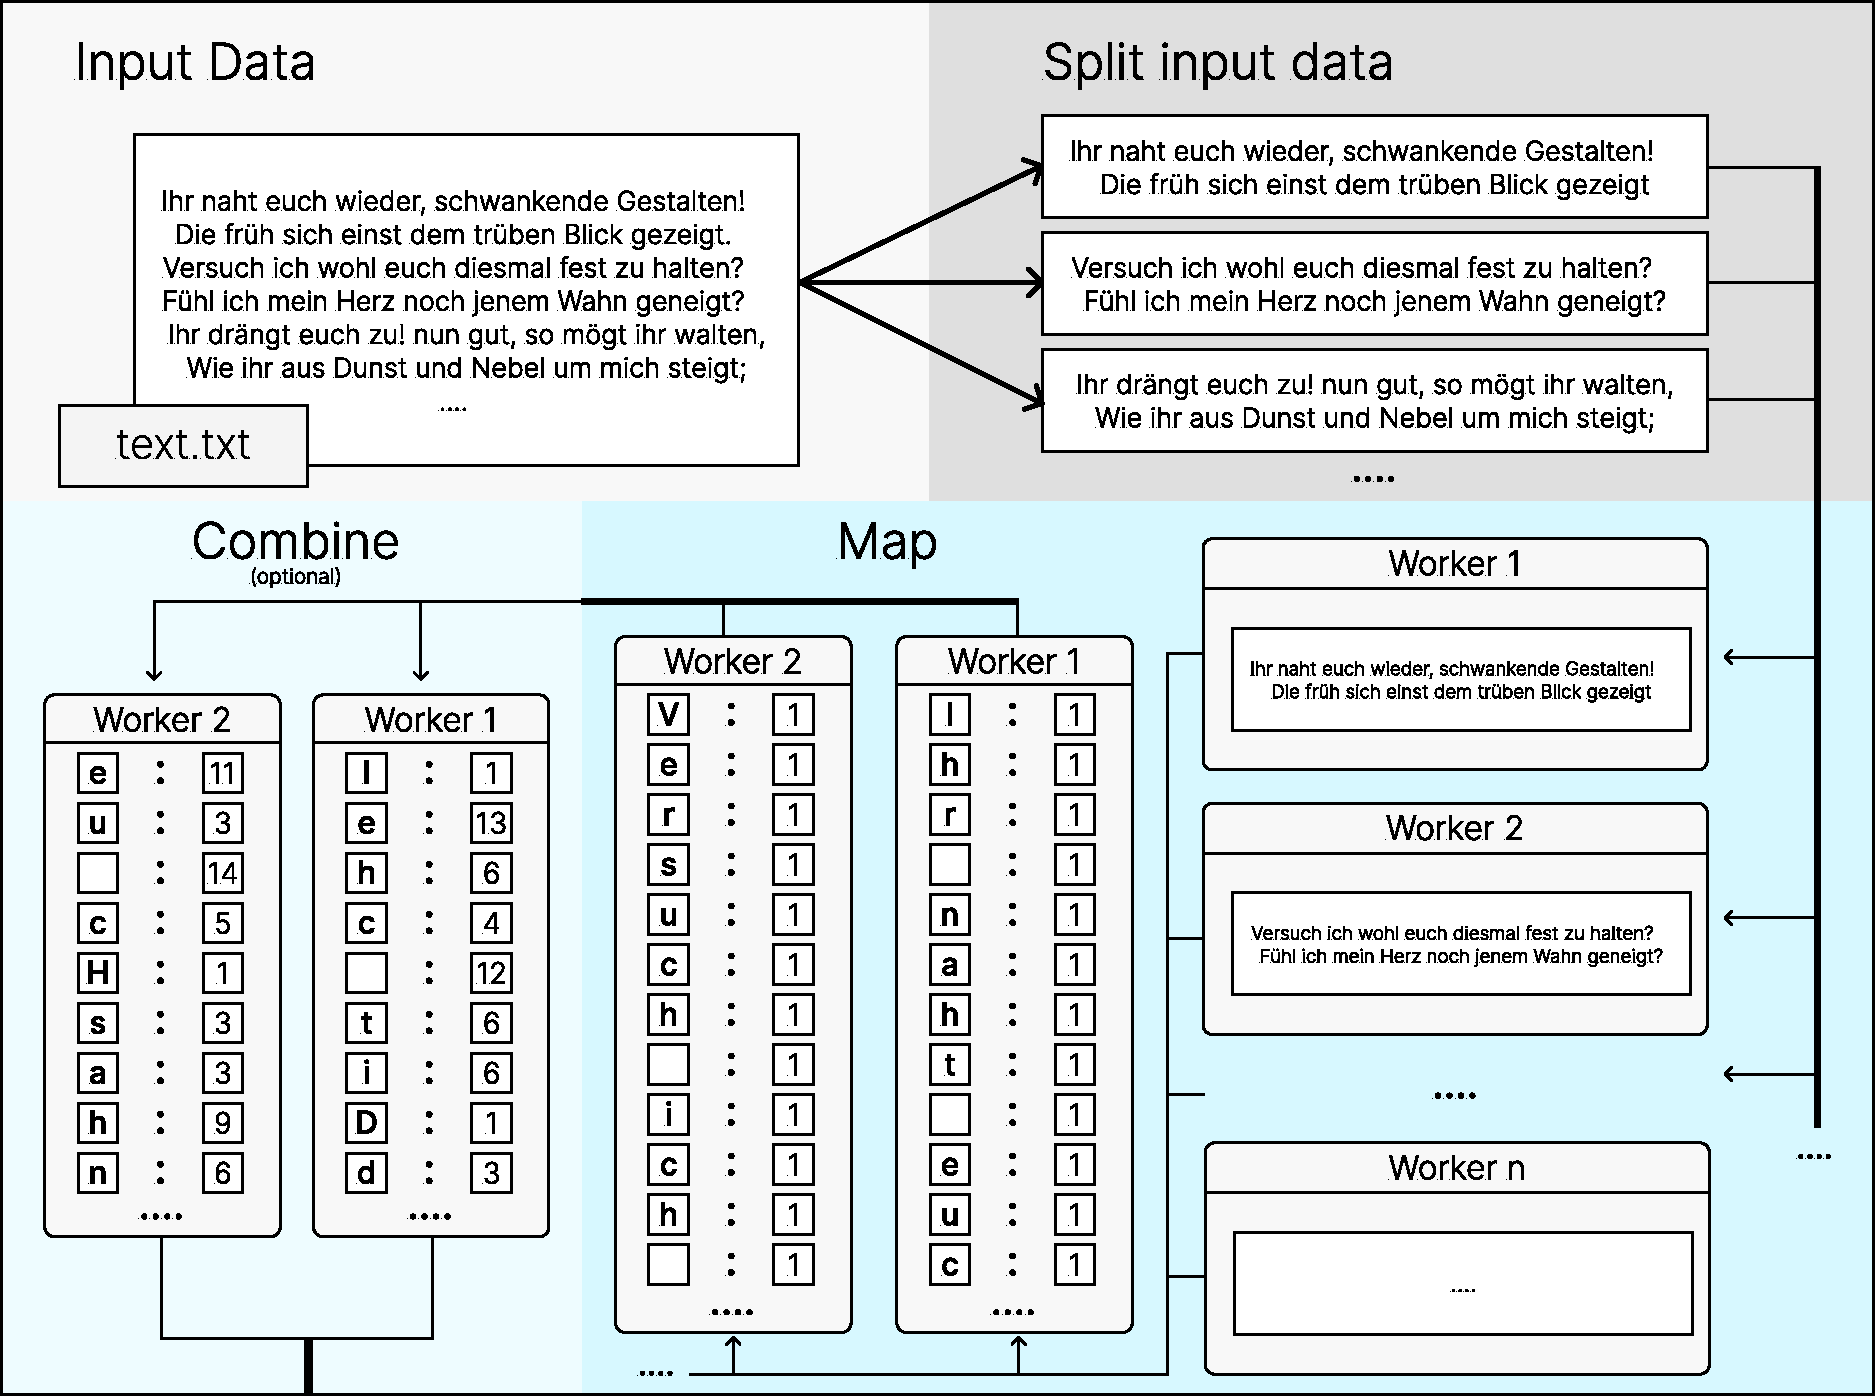
\includegraphics[width=0.9\linewidth]{img/MapReduceAblaufPart1}
	\caption{Procedure of a MapReduce operation. The use-case depicted in this example represents one of two possible applications provided by the system developed as part of this project. Continued in figure \ref{fig:mapReduceProcess2}.}
	\label{fig:mapReduceProcess1}
\end{figure}

Upon receiving the data to be processed, it needs to be split up into chunks to be assigned to workers. Splitting vast amounts of data has to be kept as simple as possible. By reducing the complexity of dividing the input data, performance is increased because the advantage of distributed computation is better utilized.\newline
Individual data chunks then get sent to workers, which process the mapping phase. After receiving the data, which in this case takes the shape of a string, the workers execute the user-defined mapping function for the given input. In this example, the resulting key/value pairs represent individual characters and the number of occurrences.\newline
Due to the nature of this application, the result after mapping the input data are a vast amount of key/value pairs. To decrease network load, a combine phase is being performed. The combine phase acts as a preliminary reduce phase for the individual workers. Depending on the number of duplicates present in the input data, the combine operation can decrease the key/value pair bundle to a fraction of the original size, further increasing performance. 

\begin{figure}[h]
	\centering
	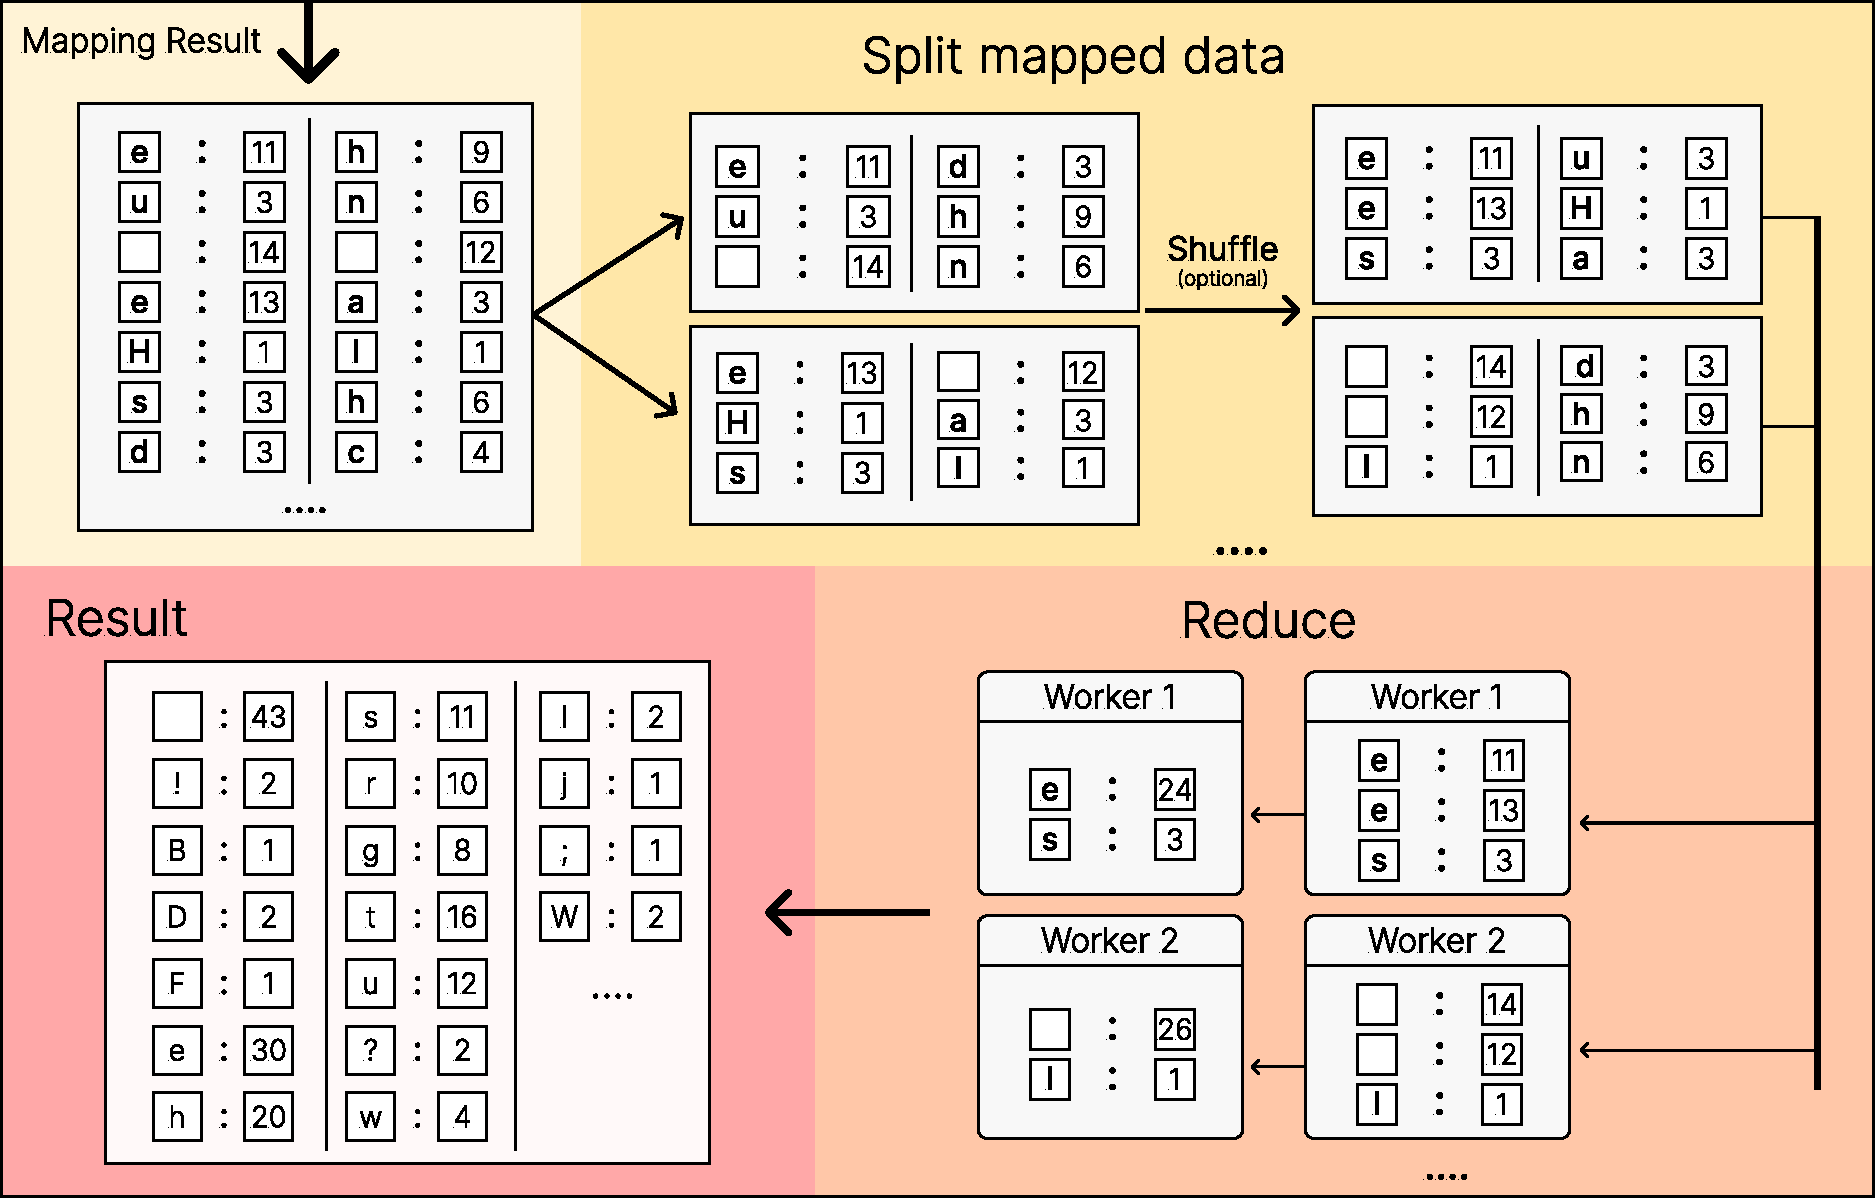
\includegraphics[width=0.9\linewidth]{img/MapReduceAblaufPart2}
	\caption{Procedure of a MapReduce operation. Continuation of figure \ref{fig:mapReduceProcess1}.}
	\label{fig:mapReduceProcess2}
\end{figure}

Each worker sends their mapping result to the master, where the results get accumulated. Once every worker has finished, the master initiates the second phase. Similar to the mapping phase, the accumulated results must be divided up into chunks and distributed to available workers. The data chunks get shuffled to guarantee the most optimal outcome from the reduce phase. The shuffle phase ensures that pairs with the same key get grouped into the same data chunk. If no shuffling is performed, the risk of the split data consisting of only heterogeneous keys remains. This would result in the reduce phase having little to no effect on decreasing the number of key/value pairs.\newline
Upon receiving mostly homogeneous data, the worker executes the user-defined reduce function. In this example, the value of pairs with similar keys gets aggregated. The extant key/value pairs then get sent to the master.\newline
The result of this application being the number of character occurrences in a given input string.

\pagebreak
\section{Classes}

The class structure in this project is oriented in the MapReduce solution Disco\footfullcite{discoDoc}. In contrast to the realization, disco provides, only three parties are present in this project. Disco uses a central master to act as an interface between the client and the workers, which are referred to as slaves in disco. Additionally, disco has a server role. This server manages several workers and acts as an intermediary between the worker and master. However, the role of the server has not been realized in this implementation to steer away from high complexity and enable the realization of a reliably working model in the time span of this project.

\subsection{Master}

The master acts as an interface connecting the clients to workers. Additionally, the master acts as the central server accepting and managing all connections. To simplify handling these tasks, the master is supported by the ClientManager and WorkerManager. These run as independent threads and allow for a delimited program structure.

\begin{figure}[h]
	\centering
	\includegraphics[width=0.6\linewidth]{img/Master}
	\caption{Structure of the Master class.}
	\label{fig:classes_Master}
\end{figure}

Figure \ref{fig:classes_Master} depicts the structure of the Master class. The master contains instances of ClientManager and WorkerManager, which run separately and take care of the tasks the master needs to handle. This leaves the core master class with an acceptConnection method, which asynchronously accepts asio clients, which are then delegated to either the WorkerManager or ClientManager.    


\subsubsection{ClientManager}

The ClientManager handels MapReduce client connections. The client refers to a human user of the MapReduce system. 

\begin{figure}[h]
	\centering
	\includegraphics[width=0.7\linewidth]{img/ClientManager}
	\caption{Structure of the ClientManager class.}
	\label{fig:classes_ClientManager}
\end{figure}

For the master to be able to add connections, the ClientManager provides a $join$ function. To support disconnecting clients, a $leave$ function is available. These functions take an instance of a connection represented by a shared pointer on a connection object. This means the ClientManager can keep track of ongoing client-master connections and act as a communication interface between them.\newline 
Additionally the $registerJob$ and $sendResult$ function are depicted in figure \ref{fig:classes_ClientManager}. These two functions handle job management on the client-side of the master. Thereby ongoing jobs are being tracked, and upon finishing, the client gets sent the resulting data. Lastly, the class contains a $generateID$ function, which generates unique ids to identify clients.

\subsubsection{WorkerManager}

The WorkerManager works analogously to the ClientManager, whereas the WorkerManager handles the master-worker communication. The WorkerManager also provides $join$ and $leave$, which are used by the master to delegate connections.  

\begin{figure}[h]
	\centering
	\includegraphics[width=0.8\linewidth]{img/WorkerManager}
	\caption{Structure of the WorkerManager class.}
	\label{fig:classes_WorkerManager}
\end{figure}

Similar to the ClientManager, the WorkerManager provides a $assignJob$ function. This function acts as the interface between the ClientManager and WorkerManger. The functionality of distributing a job received from a client is thereby realized. To allow for results to be forwarded to the WorkerManager, the functions $mapResult$ and $reduceResult$ exist. These methods are used by the ConnectionSession, where communication takes place.\newline
To increase fault-tolerance, WorkerManager provides a $reAssignTask$ function, which is used when a worker fails to perform its task correctly. The $generateID$ function works the same as in the ClientManager and is used to identify workers uniquely.  

\subsection{Client}

The Client class represents the link between the user and the MapReduce system. It implements a user interface to enable the user to communicate with the system and place job requests. 

\begin{figure}[h]
	\centering
	\includegraphics[width=0.6\linewidth]{img/Client}
	\caption{Structure of the Client class.}
	\label{fig:classes_Client}
\end{figure}

In order to initiate the connection to the master server, the ClientManager implements a $signOn$ function. Similarly, the class also provides a $signOff$ function to terminate the connection. The function $sendJob$, which is depicted in figure \ref{fig:classes_Client} is used to place job request. To enable visualization of job results, the functions $printResultsPlain$ as well as $printResultsHistogram$ are implemented by the ClientManager.The Client class represents the link between the user and the MapReduce system. It implements a user interface to enable the user to communicate with the system and place job requests. 

\subsection{Worker}

The Worker is the powerhouse of the MapReduce system. It handles the computation of tasks that are assigned by the master. For this purpose, the Worker implements the functions $handleMap$ and $handleReduce$, which can theoretically be replaced by any logic accepting and returning the same data types as MapReduce intends. 

\begin{figure}[h]
 	\centering
 	\includegraphics[width=0.8\linewidth]{img/Worker}
 	\caption{Structure of the Worker class.}
 	\label{fig:classes_Worker}
\end{figure}

The $handleMap$ and $handleReduce$ functions take the type of job, data, and job id as parameters. Whereas the $handleMap$ function accepts the raw data in the shape of a string, the $handleReduce$ function is provided with a set of key/value pairs.\newline
To control the connection to the master, the functions $signOn$ and $signOff$ are provided, which work analogously to the functions in the ClientManager.

\section{Helper Classes}

\subsection{Pipe}

To centralize the asio network connection, the pipe class is used. It provides a network interface to simplify sending and receiving messages. The pipe uses an asio socket to transfer messages. Additionally, the class ensures the thread-safe access to the socket. 

\begin{figure}[h]
	\centering
	\includegraphics[width=0.55\linewidth]{img/Pipe}
	\caption{Structure of the Pipe class.}
	\label{fig:classes_Pipe}
\end{figure}

\subsection{ConnectionObject}

To represent the client and worker connections, the ConnectionObject is used. It provides structure for connections and stores vital information used for handling ongoing connections. 

\begin{figure}[h]
	\centering
	\includegraphics[width=0.6\linewidth]{img/ConnectionObject}
	\caption{Structure of the ConnectionObject class.}
	\label{fig:classes_ConnectionObject}
\end{figure}

To identify a ConnectionObject, it contains an id, as depicted in figure \ref{fig:classes_ConnectionObject}. This id is not unique across all ConnectionObjects due to the distinction between worker and client connections. Additionally, the ConnectionObject stores information about the state of availability. However, this attribute is only used in worker connections.\newline
In an effort to increase fault-tolerance and detect broken connections the ConnectionObject stores the time, when the last message was received. It enables the server to periodically check connections and end them if no response has been received.

\subsection{ConnectionSession}

The ConnectionSession handles the communication between the master and workers as well as clients.
The basic structure of implementing asio, multi-user communication this way, has been inspired by the asio-documentation\footfullcite{asioMultiuser}.

\begin{figure}[h]
	\centering
	\includegraphics[width=0.6\linewidth]{img/ConnectionSession}
	\caption{Structure of the ConnectionSession class.}
	\label{fig:classes_ConnectionSession}
\end{figure}

To start the process of receiving and sending messages the ConnectionSession provides a $start$ function. Additionally the ConnectionSession implements the functions $sendMessage$, $isConnected$ and $closeConnection$ from the ConnectionObject class.  

\subsection{Job}

The Job class allows for uniform structure when processing jobs.

\begin{figure}[h]
	\centering
	\includegraphics[width=0.6\linewidth]{img/Job}
	\caption{Structure of the Job class.}
	\label{fig:classes_Job}
\end{figure}

Job provides a variety of constructors to simplify using the Job class in all phases of the MapReduce process. It contains an id that is unique across all jobs to identify jobs. Furthermore, a job stores information about the type of job and current status. The different states of a job are defined in the $JobStatus$ enum, depicted in figure \ref{fig:classes_JobStatus}.

\begin{figure}[h]
	\centering
	\includegraphics[width=0.3\linewidth]{img/JobStatus}
	\caption{Enum containing job states.}
	\label{fig:classes_JobStatus}
\end{figure}

\subsubsection{ActiveJob}

To allow for tasks to be reassigned upon failure, the ActiveJob class provides all information.
Due to the reciprocal relationship between ActiveJob and Job, it is necessary to split the ActiveJob into two classes. The class ActiveJob, depicted in figure \ref{fig:classes_ActiveJob} is the derived from the class ActiveJobStruct, depicted in figure \ref{fig:classes_ActiveJobStruct}.

\begin{figure}[h]
	\centering
	\includegraphics[width=0.28\linewidth]{img/ActiveJob}
	\caption{Structure of the ActiveJob class.}
	\label{fig:classes_ActiveJob}
\end{figure}

The class ActiveJobStruct provides the structure of an active job. Thereby information on all phases of the MapReduce process is stored in an ActiveJob. Additionally, to the attributes contained in the Job class, it also allows storing the data each worker is currently processing.

\begin{figure}[h]
	\centering
	\includegraphics[width=0.7\linewidth]{img/ActiveJobStruct}
	\caption{Structure of the ActiveJobStruct class.}
	\label{fig:classes_ActiveJobStruct}
\end{figure}
\pagebreak

\subsection{MessageQueue}

Due to communication taking place between multiple parties, it is crucial to serialize the processing of messages. This concept can be realized by using a queue, in this project realized through the MessageQueue class, depicted in figure \ref{fig:classes_MessageQueue}.

\begin{figure}[h]
	\centering
	\includegraphics[width=0.5\linewidth]{img/MessageQueue}
	\caption{Structure of the MessageQueue class.}
	\label{fig:classes_MessageQueue}
\end{figure}

To implement the functionality of a queue, MessageQueue uses the queue data type provided by c++. Additionally, MessageQueue ensures that access to the queue happens in a thread save manner. 

\subsubsection{QueueItem}

To store the data of an item in the queue, the QueueItem class provides the needed structure. 
The QueueItem stores data that can be received by the master from workers.

\begin{figure}[h]
	\centering
	\includegraphics[width=0.55\linewidth]{img/QueueItem}
	\caption{Structure of the QueueItem class.}
	\label{fig:classes_QueueItem}
\end{figure}

\subsection{MessageGenerator}

To simplify working with protobuf messages, the MessageGenerator provides various functions that return the respective message. 

\begin{figure}[h]
	\centering
	\includegraphics[width=0.90\linewidth]{img/MessageGenerator}
	\caption{Structure of the MessageGenerator class.}
	\label{fig:classes_MessageGenerator}
\end{figure}

\pagebreak
\section{Class-diagram}

\begin{figure}[hp]
	\centering
	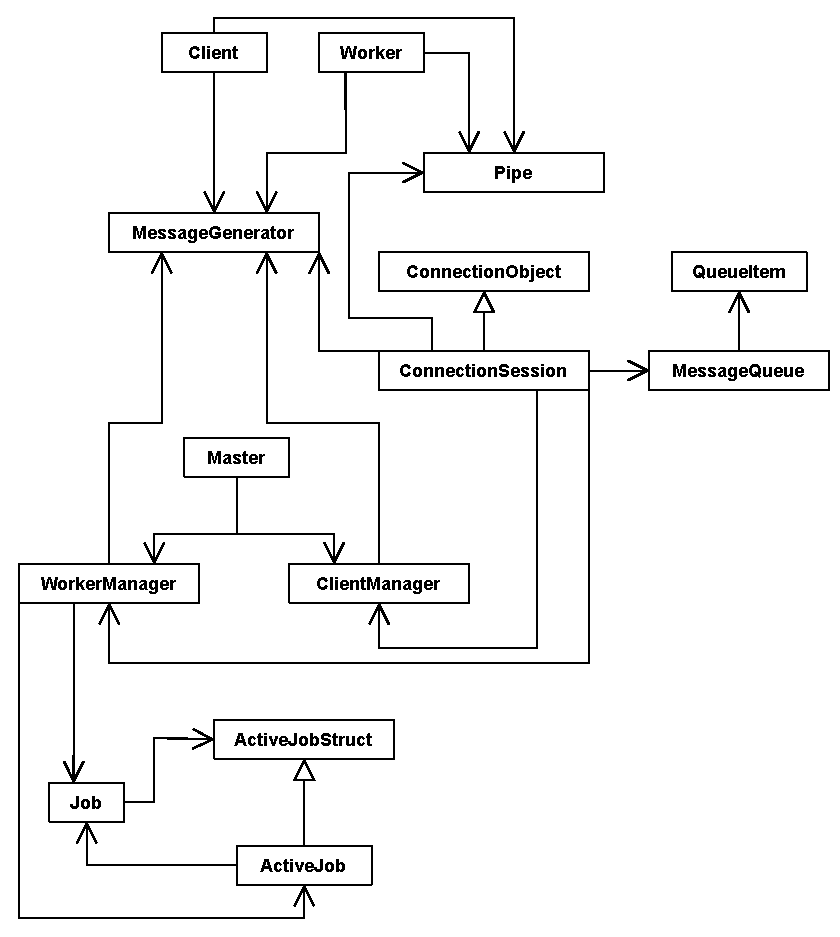
\includegraphics[width=0.75\linewidth]{img/ClassDiagram}
	\caption{UML class diagram representing the structure of this project.}
	\label{fig:classDiagram}
\end{figure}

\section{Network communication}

\subsection{protobuf}

Protobuf is used to send structured data over an asio TCP connection. In this project, the version proto3 is being used. Protocol Buffers allow for defining the structure of a message. This happens in a '.proto' file, which is then compiled with the help of protoc. Protobuf supports a variety of different programming languages. In the case of C++, protobuf generates header files. These contain the code necessary to instantiate predefined message objects and serialize or parse them.  

\subsection{Messages}

\subsubsection{Authentication}
An Authentication message is used to identify the type of connection. In this project, there are two possible types, client or worker. Upon successfully connecting to the master, an Authentication with the respective connection type is sent. 

\subsubsection{Assignment}
The Assignment message is used to assign ids to workers and clients. An Assignment is sent in the ConnectionSession after a new connection gets accepted by the master. It contains the id that the connection partner gets assigned and the type of connection, either client or worker.

\subsubsection{SignOff}
A SignOff message is either sent from a worker or client upon encountering an error that results in the program's termination. This is performed to let the master know when a client or worker is no longer available. The SignOff message can also be sent from master to client or worker to force them to stop. This behavior can be observed when the master program terminates. A SignOff contains the id of client or worker that is about to disconnect and the respective connection type.

\subsubsection{Confirm}
A Confirm is used the ensure that important messages have been delivered. An example of its application is to confirm that an Assignment has been delivered. This is especially important because all later communication is based on ids. If a client or worker has not been assigned an id, it would not be possible for future messages to be accepted by the master due to the lack of identification of the sender. 

\subsubsection{TaskMap}
The TaskMap message gets sent from master to worker to assign a task to the respective worker along with the needed information to perform it. The message contains the job id, which uniquely identifies the job. This represents essential information to match the result sent by the worker to the original job. Furthermore, the type of job and data is being transferred.

\subsubsection{TaskReduce}
The TaskReduce message works analogously to the TaskMap message. However, instead of the data consisting of a string, that being the case with TaskMap, in TaskReduce, the data gets transferred in the shape of key/value pairs. 

\subsubsection{ResultMap}
ResultMap is a message that is sent by the worker upon finishing the mapping task. It contains the mapping result in the form of key/value pairs. Furthermore, it contains the job id to enable the master to match tasks to jobs.

\subsubsection{ResultReduce}
ResultReduce gets sent by the worker upon finishing the reduce task. The result is transferred in the shape of key/value pairs. Additionally, it contains the id of the job. 

\subsubsection{JobRequest}
A JobRequest is sent from client to master. It contains information on the job to be performed and the data to be processed. Furthermore, the client can specify the number of mapping workers and reducing worker it desires. 

\subsubsection{JobResult}
The JobResult is the reply to the client from the master after finishing the job. It contains the result of the MapReduce operation in the form of key/value pairs.  

\subsubsection{Ping}
The Ping message is used for checking connections. After the master detects a worker being inactive for an extended period of time it sends pings in one-second intervals until a reply is received or five pings have been sent. If a worker receives a Ping, it replies with a Ping message.

\subsection{Sequence Diagram}

\begin{figure}[h]
	\centering
	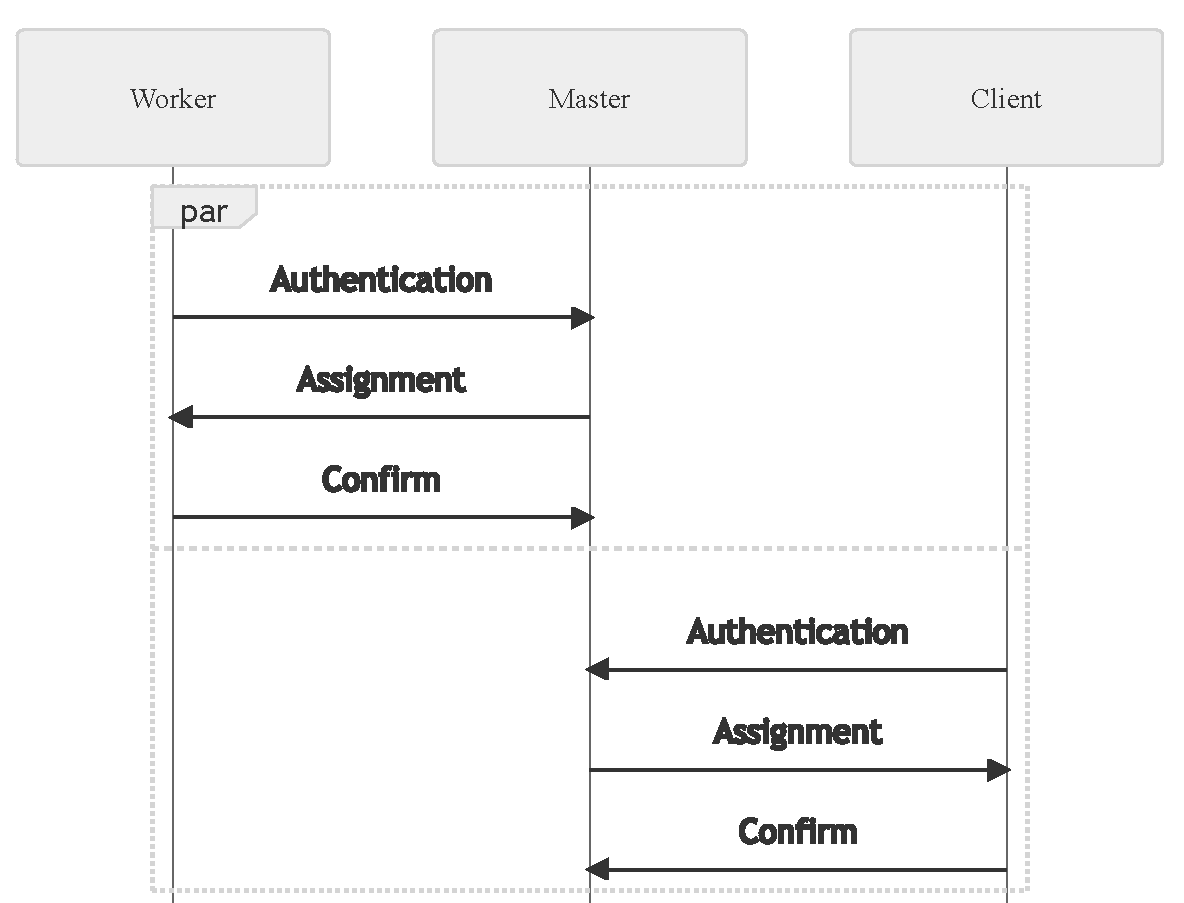
\includegraphics[width=0.6\linewidth]{img/SequenceDiagramPart1}
	\caption{Sequence diagram depicting the network traffic of the MapReduce system. Continued in figure \ref{fig:sequenceDiagramPart2}}
	\label{fig:sequenceDiagramPart1}
\end{figure}

\begin{figure}[hp]
	\centering
	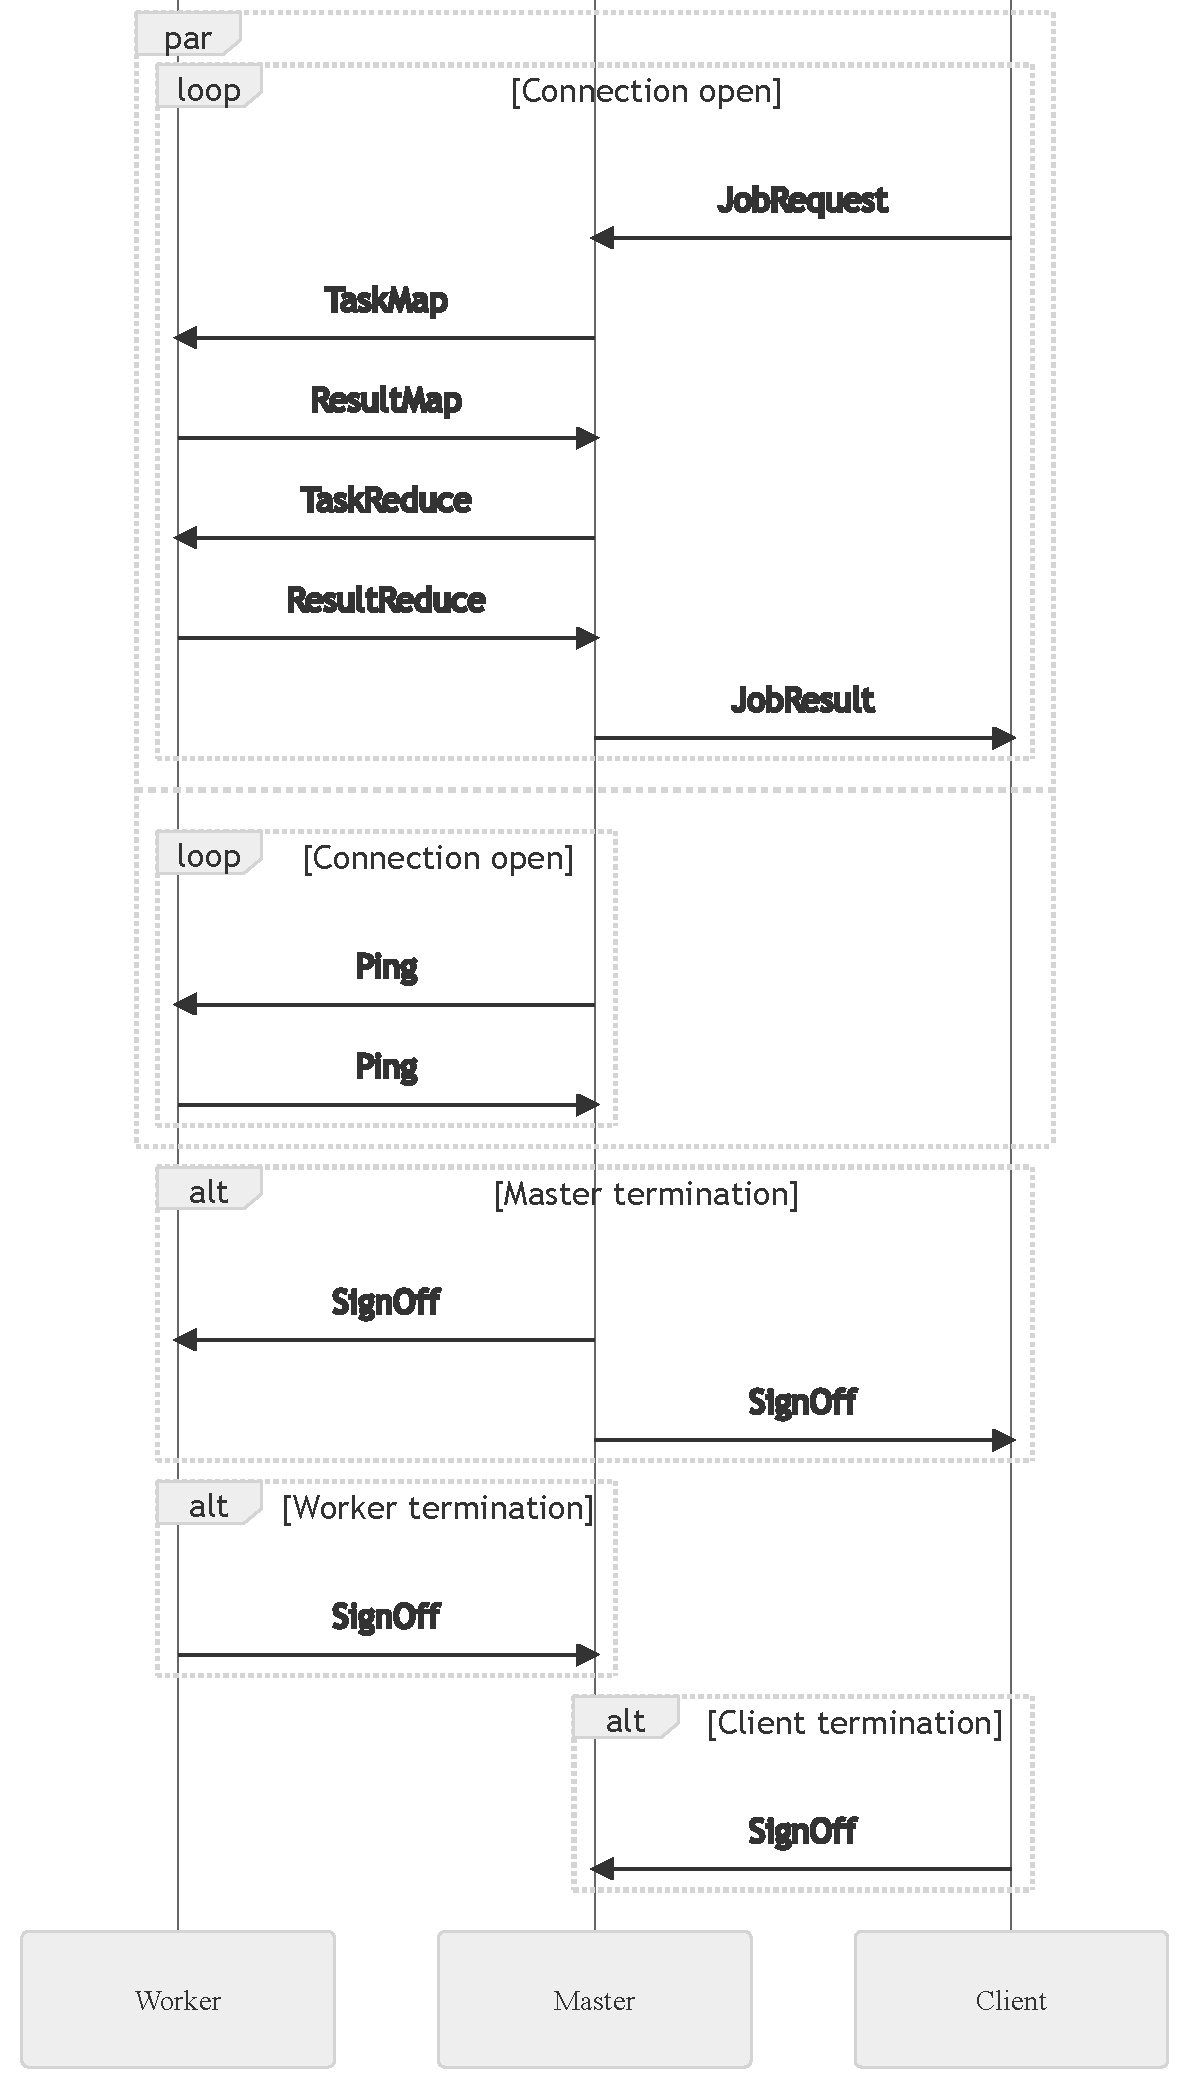
\includegraphics[width=0.75\linewidth]{img/SequenceDiagramPart2}
	\caption{Sequence diagram}
	\label{fig:sequenceDiagramPart2}
\end{figure}

\section{Parallelization and fault-tolerance}

The characteristic of a MapReduce system is its ability of parallel and fault-tolerant processing. This is also, to an extent, realized in this project.\newline
Upon starting a MapReduce master it accepts a variable amount of workers and clients. If a client places a job request while no workers are available, then the job gets queued by the WorkerManager and assigned to workers when available. This allows multiple clients to place jobs simultaneously without discarding jobs unable to process at the current time.\newline
The premise of MapReduce being distributed computation of one whole operation is vulnerable to failing at the weakest link in the chain. To prevent this from happening, the master can reassign failed tasks. These failed tasks behave the same as jobs. If no workers are currently available, they get queued. In the case of multiple tasks failing from the same job, they get merged into one job and distributed to workers once available.\newline
There are different reasons why a worker fails his task. The easiest for the master to detect is if a SignOff message is received from a worker that is currently assigned a task. If the worker is unable to communicate over the network, the master will timeout the connection after 15 seconds since the last response and reassign the task. 

\section{Usage}
\label{usage}

To use MapReduce, clone the repository Kleinrad/kleinrad\_project\footfullcite{mapreduceRepo}. After all dependencies listed in section \ref{libraries} are satisfied, compile the project via meson. To ensure a successful build use meson 0.59.1+. Once compiled the three executables have been generated: $mr\_worker$, $mr\_master$, and $mr\_client$.\newline
Start the $mr\_master$, which then will wait for incoming connections. After that, it is possible to start as many $mr\_worker$s and $mr\_client$s as needed. To place a request, use the command line interface provided by the client.

\pagebreak
\subsection{Command Line}
The Client supports a variety of command-line arguments and commands.

\subsubsection{Arguments} 
\begin{itemize}
	\item [\textbf{ip}] - specify ip-address of MapReduce master 
	\item [\textbf{port}] - specify MapReduce port
\end{itemize} 

\subsubsection{Commands}
Furthermore, the client provides a command-line interface to place job requests and display job results. The available commands consist of:

\begin{itemize}
	\item [\textbf{help}] - print available commands, along with parameters
	\item [\textbf{quit}] - end client session
	\item [\textbf{send}] - send a job request
	\item [\textbf{print}] - print last job results
\end{itemize}

The $send$ and $print$ commands accept parameters to specify the request further.

\begin{itemize}
	\item [\textbf{send}] $<jobType>\ [-f]\ <data>$
\end{itemize} 

The job type can either be 0 or 1. These represent different reduce operations.
Job type 0 counts the number of character occurrences, whereas job type 1 counts the number of word occurrences. The optional parameter $-f$ can be used to provide a txt file as the input data. If the parameter $-f$ is non-existent, the $data$ can be a string of variable length.\newline
To display the results returned to the client, the $print$ command can be used.
\begin{itemize}
	\item [\textbf{print}] $[-s]\ <printType>$
\end{itemize}  
The print command has the optional parameter $-s$. Thru the use of this parameter, the output will be sorted by the value of the results. Furthermore, the print command requires a $printType$ to be specified. This can either be 0 or 1. Print type 0 returns a list containing the results of the last job, along with the percentage share per occurrence relative to the whole input text. Print type 1 prints the results as a Histogram. 


\subsubsection{Configuration}
The configuration is performed via json. To use json in c++ the nlohmann json library\footfullcite{nlohmannJson} is used. With this json file, the port of the master and the ip and port a worker connects to are specified.

\section{Libraries}
\label{libraries}
\begin{table}[h]
	\centering
	\begin{tabular}{l|l}
		Purpose                       & Technology \\ \hline
		Build Tool				 	  & Meson 	   \\
		Command line interface	      & CLI11      \\
		Configuration files           & json       \\
		Data serialization            & protobuf   \\
		Logging                       & spdlog     \\
		Network Communication         & asio       \\
		Programming Language		  & C++ 17 \\
	\end{tabular}
	\caption{In this table used external technologies are listed.}
\end{table}

\newpage

\section{Project Structure}
\dirtree{%
	.1 /.
	.2 LICENSE.
	.2 meson\_options.txt.
	.2 meson.build.
	.2 README.md.
	.2 CHANGELOG.org.
	.2 config.json.
	.2 include.
	.3 client.h.
	.3 clientmanager.h.
	.3 connectionobject.hpp.
	.3 connectionsession.h.
	.3 job.hpp.
	.3 master.h.
	.3 messageQueue.hpp.
	.3 pipe.hpp.
	.3 protoutils.hpp.
	.3 worker.h.
	.3 workermanager.h.
	.2 src.
	.3 Message.proto.
	.3 client.hpp.
	.3 clientmanager.hpp.
	.3 connectionsession.cpp.
	.3 master.cpp.
	.3 worker.cpp.
	.3 workermanager.cpp.
	.2 doc.
	.3 doc.pdf.
	.3 doc.tex.
	.3 references.bib.
	.2 build.
}\hfill

% .bib include & references
\newpage

\printbibliography
\end{document}